\subsection{The Physics of Optical Communications}

Optical communications systems utilise light, typically provided by laser
diodes, or LED's, in order to transmit information along an optical fiber cable.
The optics principle of total internal reflection is utilised for the purpose of
transmission. When the incident angle of the light in the cable is greater than
the critical angle at the ``core-to-cladding interface''\cite{alwayn_2004}, the
light will reflect back into the core. This repeats thoughout the fibers core,
passing the light from source to destination.

\begin{figure}[H]
	\centering
	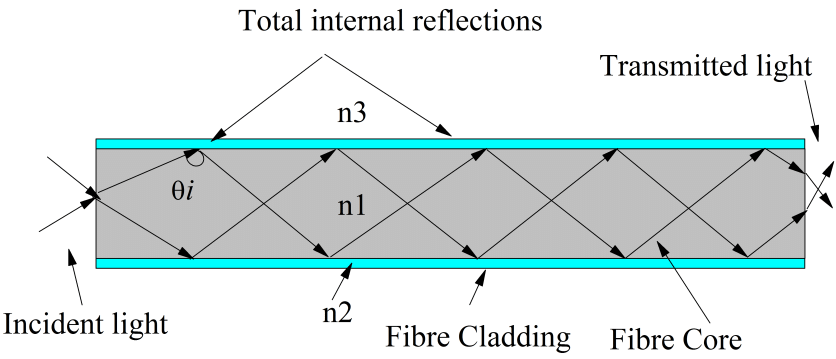
\includegraphics[width=0.8\textwidth]{images/tir}
	\caption{Total Internal Reflection within an Optical Fiber
	Cable\cite{memon_2018}}
	\label{fig:tir}
\end{figure}

\par Optical communications systems utilise light in the infrared spectrum to pass
information along a cable. The wavelength of the light in this spectrum is
in the order of thousands of micrometers ($\mu m$) in length, with frequencies
in the order of hundreds of terahertz ($\approx 10^{13}Hz$). These
high-frequency, low-wavelength carrier signals result in very high bandwidths,
and very high data transfer rates\cite{mickelson_2003}.

\par The directionality of laser light within these systems allows for greater
efficiency, as energy is not required for the filtering or correction of
divergent beams\cite{mickelson_2003}.
